\documentclass[a4paper,10pt]{article}

\usepackage[T1]{fontenc}
\usepackage[utf8]{inputenc}
\usepackage[brazil]{babel}

\usepackage{geometry}
\geometry{
    textwidth=190mm,	
    textheight=267mm,	
	inner=10mm,		
	outer=10mm,		
	top=10mm,
	bottom=20mm
}
\usepackage{fancyhdr}
\usepackage{graphicx}
\usepackage{fontawesome}
\usepackage{hyperref}
\hypersetup{
	colorlinks = true,
	urlcolor = cyan,
	linkcolor = black,
}

%%%%%%%%%%%%%%%%%%% - Alterações de Uso - %%%%%%%%%%%%%%%%%%%
\newcommand{\profissional}{Mateus Souza Oliveira}
\newcommand{\idade}{24}
\newcommand{\Endereco}{Rodovia Amaro Antônio Vieira, 2593 -- Itacorubi. Florianópolis, Santa Catarina, Brasil}
\newcommand{\telefone}{+55 (48) 9 9810-2694}
\newcommand{\email}{matews1943@gmail.com} 
\newcommand{\data}{24 de setembro de 2020}
\newcommand{\sobre}{
    Pró-ativo, detalhista, determinado e sempre em busca de me aprimorar. Em busca da minha primeira oportunidade como desenvolvedor júnior! Atualmente, estou estudando programação e cursando o mestrado em Matemática Pura e Aplicada na Universidade Federal de Santa Catarina (UFSC). Desejo ter contato com as diferentes áreas da profissão, com objetivo de descobrir qual combina mais com meu perfil. Já fiz projetos web com Python, HTML, CSS e JavaScript (disponíveis no meu repositório do GitHub).
    \vspace{0\baselineskip}
}
%%%%%%%%%%%%%%% - Fim de Alterações de Uso - %%%%%%%%%%%%%%%%

\setlength{\fboxrule}{2pt}
\setlength{\fboxsep}{0pt}

\fancyhead{} % Cabeçalho: reset
\fancyfoot{} % Rodapé: reset
\fancyfoot[C]{Página \thepage \ de \pageref{ultimaPagina}} % Rodapé: centro
\fancyfoot[R]{Feito com \LaTeX} % Rodapé: direito
\fancyfoot[L]{Atualizado em \data} % Rodapé: esquerdo
\renewcommand{\headrulewidth}{0pt} % Espessura da linha de cabeçalho
\renewcommand{\footrulewidth}{0.4pt} % Espessura da linha de rodapé
\pagestyle{fancy} % Define o estilo da página

\newcommand{\criaSecao}[4][0]{
    \noindent
	\begin{minipage}{0.16\linewidth}
		\large{\textbf{#2}}
		\vspace{#3\baselineskip}
	\end{minipage}
	\hfill
	\begin{minipage}{0.79\linewidth}
		#4
		\ifnum0#1>0 { \hrule {\ } } \fi
	\end{minipage}
	\vspace{\baselineskip}
}

\begin{document}
	
	\noindent
	\fbox{
	\hspace*{-3.35\fboxrule}
	\begin{minipage}{0.3\linewidth}
		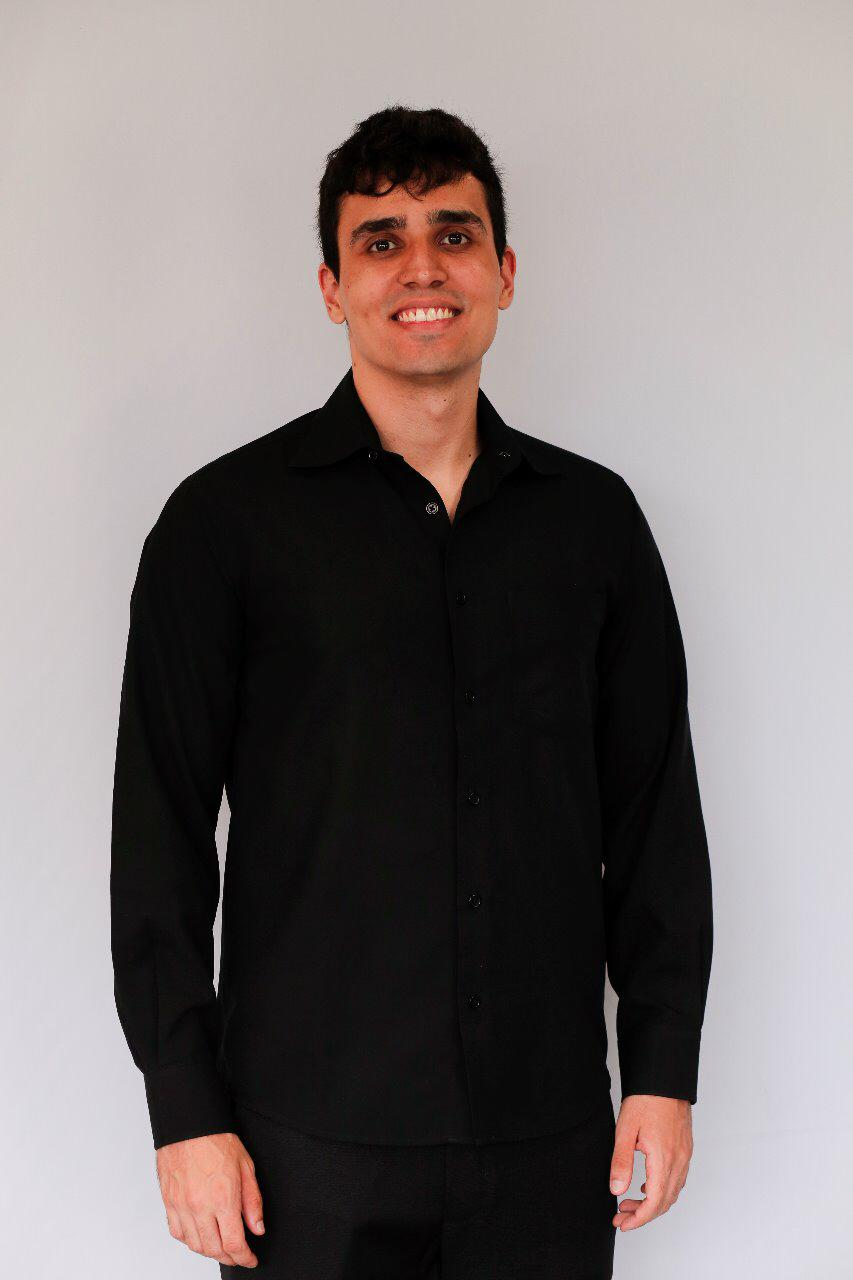
\includegraphics[width=\linewidth]{Imagens/perfil.jpeg}
	\end{minipage}
	\hspace*{-3.35\fboxrule}
	}
	\hfill
	\begin{minipage}{0.65\linewidth}
		\Huge{\bf \profissional, \idade}\\\vspace{-1.75\baselineskip}
		
		\noindent\rule{\textwidth}{1.5pt} {\ }\\\vspace{-1.8\baselineskip}
		
		\large{
		\faMapMarker \ \Endereco \\
		\begin{minipage}{0.5\linewidth}
			\faWhatsapp \ \telefone
		\end{minipage}
		\begin{minipage}{0.5\linewidth}
			\faEnvelope \ \email
		\end{minipage}
		\faLink \ \url{https://mateusoliveira43.github.io/}\\
		\faLinkedinSquare \ \url{https://www.linkedin.com/in/mateusoliveira43/}\\
		\faGithub \ \url{https://github.com/mateusoliveira43} \\
		\vfill
		\textbf{Sobre}: \sobre
		}
	\end{minipage}
	\vspace{\baselineskip}
	
%%%%%%%%%%%%%%%%%%%%%%% - Corpo do CV - %%%%%%%%%%%%%%%%%%%%%%%
    \criaSecao[1]{Objetivos}{3}{
        Quero trabalhar em um local onde possa sempre me aprimorar. Desejo ter contato com as diferentes áreas da profissão antes de me especializar em uma área/linguagem. Tenho interesse em trabalhar com linguagens de programação, \textit{frameworks} e ferramentas com as quais não tenha experiência prévia. Busco trabalhar no estado de Santa Catarina ou remotamente. \\
    }
    
    \criaSecao[1]{Educação}{4}{
        \textit{Pós-Graduação em Matemática Pura e Aplicada (Mestrado)}, Universidade Federal de Santa Catarina (UFSC), Florianópolis, Santa Catarina \hfill 2020 - atualmente \\
		
		\textit{Matemática - Bacharelado}, Universidade Federal de Santa Catarina (UFSC), Florianópolis, Santa Catarina \hfill 2014 - 2020 \\
    }
    
    \criaSecao[1]{Experiência}{14}{
        \textit{Bolsista de Iniciação Científica}, Universidade Federal de Santa Catarina (UFSC), Florianópolis, Santa Catarina \hfill Agosto 2019 - Fevereiro 2020 \\
		\textbf{Atividades}: Pesquisa voltada a computação gráfica.\\
		
		\textit{Bolsista do Laboratório de Estudos de Matemática e Tecnologias}, Universidade Federal de Santa Catarina (UFSC), Florianópolis, Santa Catarina \hfill Março 2019 - Julho 2019 \\
		\textbf{Atividades}: Aplicação, desenvolvimento e atualização de arquivos do projeto.\\
		
		\textit{Bolsista da Revista da Olimpíada Regional de Matemática de Santa Catarina}, Universidade Federal de Santa Catarina (UFSC), Florianópolis, Santa Catarina \hfill Março 2016 - Março 2017 \\
		\textbf{Atividades}: Aplicação e desenvolvimento de arquivos de treinamento; correção e desenvolvimento de arquivos de prova; atualização do arquivo mestre da revista.\\
		
		\textit{Bolsista do Programa de Educação Tutorial de Matemática}, Universidade Federal de Santa Catarina (UFSC), Florianópolis, Santa Catarina \hfill Março 2015 - Fevereiro 2016 \\
		\textbf{Atividades}: Aplicação e desenvolvimento de arquivos de treinamento; lecionamento em cursinho pré-vestibular; lecionamento e elaboração de minicursos de \LaTeX\ e Matlab. \\
    }
    
    \criaSecao[1]{Linguagens de programação e ferramentas}{1}{
        \large{\bf
			\begin{minipage}{0.33\linewidth}
				Python (Django)\\
				JavaScript (Node.js)\\
				Git\\
			\end{minipage}
			\begin{minipage}{0.33\linewidth}
				HTML\\
				CSS (Bootstrap)\\
				Linux\\
			\end{minipage}
			\begin{minipage}{0.33\linewidth}
				MySQL\\
				MongoDB\\
				\\
			\end{minipage}
		}
    }
	
	\criaSecao{Idiomas}{1}{
	    \large{
			\begin{minipage}{0.5\linewidth}
				\textbf{Português}: nativo \\
				\textbf{Inglês}: fluente \\
			\end{minipage}
			\begin{minipage}{0.5\linewidth}
				\textbf{Espanhol}: básico \\
				\textbf{Alemão}: básico \\
			\end{minipage}
		}
	}
%%%%%%%%%%%%%%%%%%% - Fim do Corpo do CV - %%%%%%%%%%%%%%%%%%%
\label{ultimaPagina}
\end{document}